\section{Procedure}
\label{sec:Procedure}

The first step is to find the minimal current value for the laser setup, where
it is still lasing. Therefore the cavity will be varied by the two knobs.
The minimum can be found in an iterative procedure, which follows the following
steps. First pick a current, where the laser is lasing.
Then go slightly beolow the lasing threshold and try to bring the system back to lasing,
by adjusting the cavity with the two knobs.
If this is possible, lower the current
until it is slightly below the threshold and repeat the procedure.


\begin{align}
  \label{eqn:nolase}
  I_{below} &= \SI{33.2}{\milli\ampere}\\
  I_{above} &= \SI{33.4}{\milli\ampere}
\end{align}

\begin{figure}
  \centering
  \begin{subfigure}{0.48\textwidth}
    \centering
    \includegraphics[width=\textwidth]{Pics/threshold_no_lase.jpg}
    \caption{The current is below the lasing threshold $I_{below}$.}
    \label{fig:no_lase}
  \end{subfigure}
  \begin{subfigure}{0.48\textwidth}
    \centering
    \includegraphics[width=\textwidth]{Pics/threshold_lase.jpg}
    \caption{The current is above the lasing threshold $I_{above}$.}
    \label{fig:lase}
  \end{subfigure}
\end{figure}


\begin{figure}
  \centering
  \includegraphics[width=0.5\textwidth]{Pics/Rb_florescence.jpg}
  \caption{Rubidium florescense line.}
  \label{fig:florescence}
\end{figure}

\begin{figure}
  \centering
  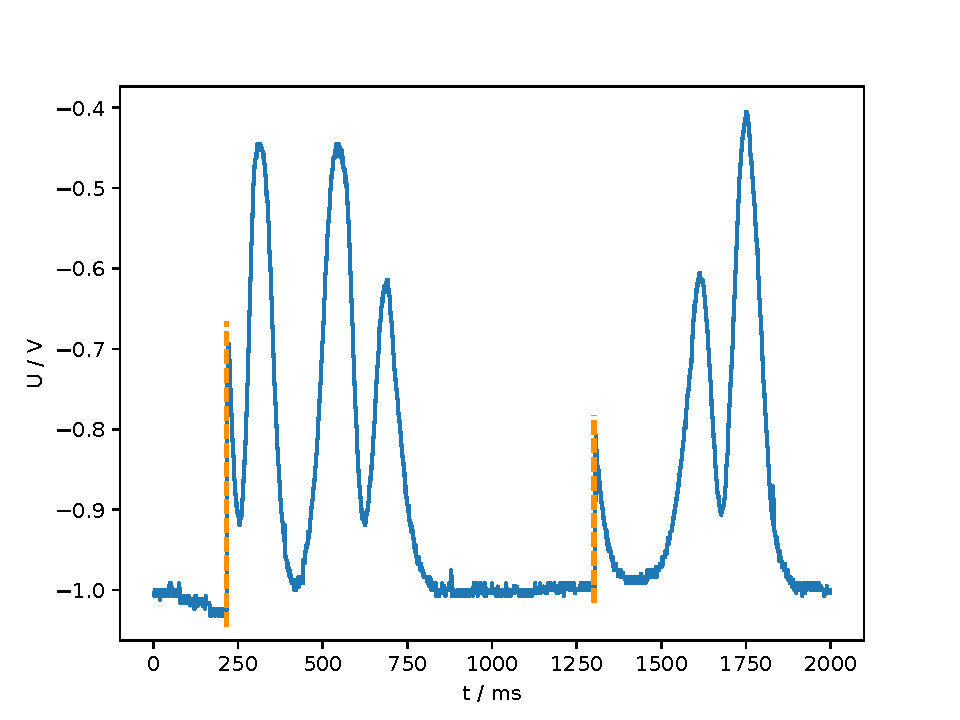
\includegraphics[width=0.7\textwidth]{Pics/example_spectrum_hop.pdf}
  \caption{Example spectrum. The mode hopes are indicated by the orange markers.}
  \label{fig:example}
\end{figure}

\begin{figure}
  \centering
  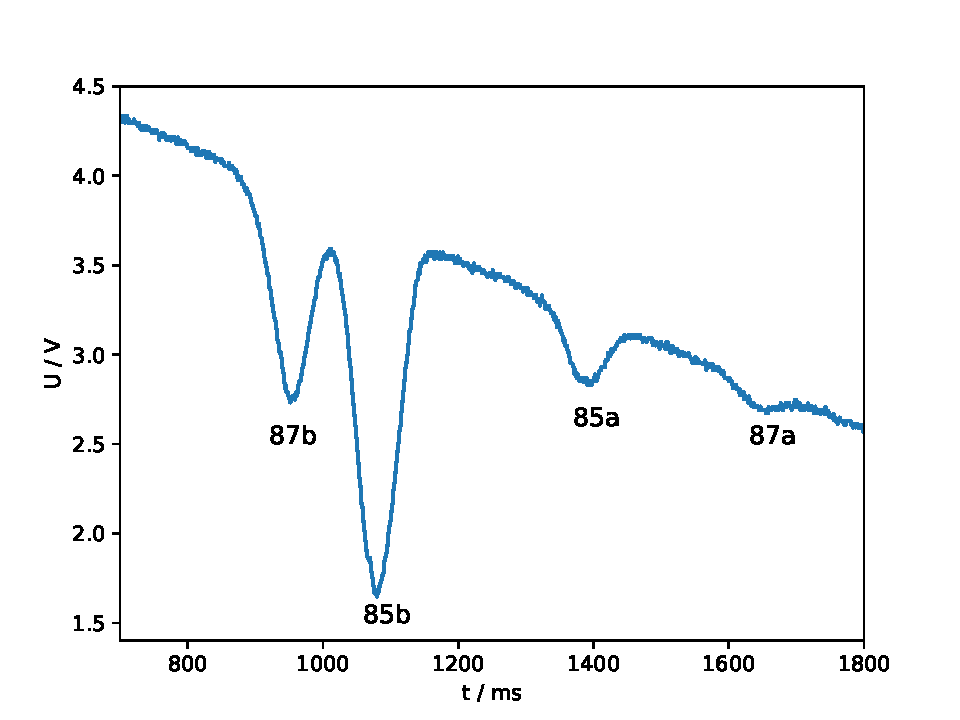
\includegraphics[width=0.7\textwidth]{Pics/Rb_spectrum.pdf}
  \caption{Rubidium spectrum.}
  \label{fig:spectrum}
\end{figure}

\begin{figure}
  \centering
  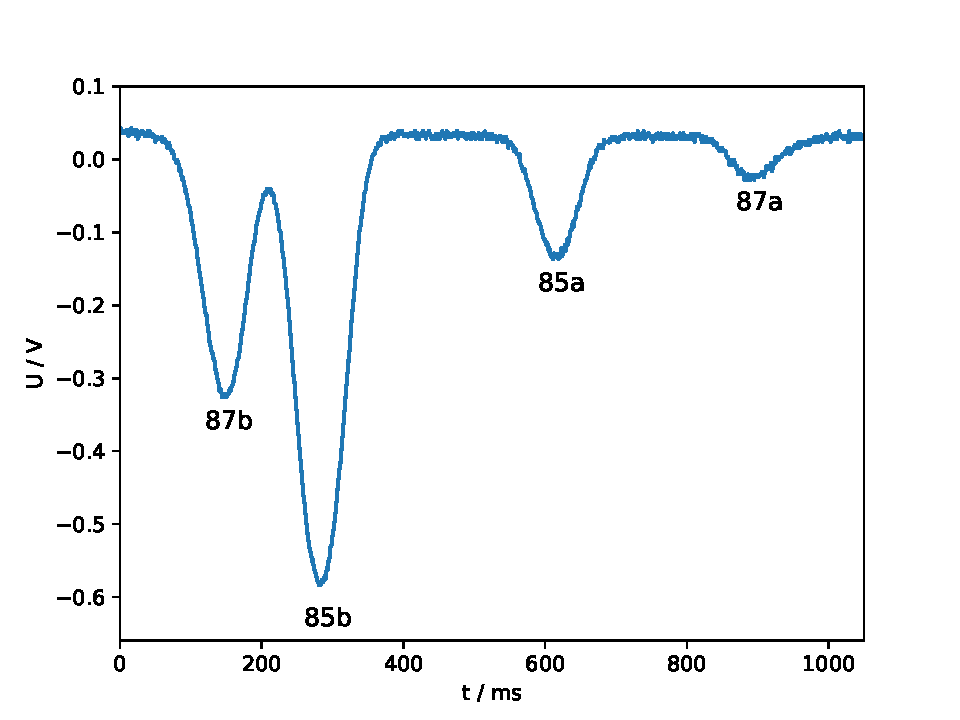
\includegraphics[width=0.7\textwidth]{Pics/Rb_spectrum_subst.pdf}
  \caption{Rubidium spectrum with substraction technique.}
  \label{fig:spectrum_sub}
\end{figure}
